% !TEX program = pdflatex
% article.tex -- LaTeX version of paper.md
% HEPDataset: A configurable framework for constructing high dimensional
% machine learning datasets from ROOT files
%
% Build:  pdflatex article && bibtex article && pdflatex article && pdflatex article
% Bibliography: paper.bib

\documentclass[11pt,a4paper]{article}

\usepackage[T1]{fontenc}
\usepackage[utf8]{inputenc}
\usepackage{newtxtext,newtxmath}
\usepackage[margin=2.5cm]{geometry}
\usepackage{amsmath}
\usepackage{graphicx}
\usepackage{booktabs}
\usepackage{array}
\usepackage{microtype}
\usepackage[font=small,labelfont=bf]{caption}
\usepackage{tikz}
\usetikzlibrary{positioning,calc,arrows,shapes.geometric}
\usepackage[round,authoryear]{natbib}
\usepackage[hidelinks]{hyperref}

\hypersetup{
  pdftitle={HEPDataset: A configurable framework for constructing high dimensional machine learning datasets from ROOT files},
  pdfauthor={A. M. M. Elsayed and Yusheng Wu},
  pdfkeywords={Python; High Energy Physics; Machine Learning}
}

% ---------------------------------------------------------------------
% shared figure styles
% ---------------------------------------------------------------------
\tikzset{
  flowbox/.style={
    draw=black!65, fill=black!3, rounded corners=2pt,
    align=center, font=\scriptsize, line width=0.4pt,
    inner xsep=3pt, inner ysep=3pt,
    text width=2.9cm, minimum height=0.85cm,
    execute at begin node={\hyphenpenalty=10000\exhyphenpenalty=10000}},
  cardbox/.style={flowbox, fill=black!13},
  hubbox/.style={flowbox, fill=black!20, text width=4.9cm},
  broadbox/.style={flowbox, text width=4.6cm},
  fl/.style={-latex, line width=0.45pt},
  flgray/.style={-latex, line width=0.45pt, black!55},
  hdrbox/.style={
    draw=black!65, fill=black!12, rounded corners=2pt, align=center,
    font=\scriptsize\bfseries, line width=0.4pt, inner xsep=2pt,
    text width=1.95cm, minimum height=0.8cm},
  msgtext/.style={
    align=center, font=\scriptsize, text width=2.45cm,
    inner sep=1.5pt, fill=white,
    execute at begin node={\hyphenpenalty=10000\exhyphenpenalty=10000}},
  selftext/.style={
    align=center, font=\scriptsize, text width=2.45cm,
    inner sep=1.5pt, fill=white,
    execute at begin node={\hyphenpenalty=10000\exhyphenpenalty=10000}},
  lifeline/.style={black!55, dashed, line width=0.4pt}
}

\newcommand{\msg}[5]{% from x, to x, y, label, style
  \draw[#5, line width=0.5pt] (#1,#3) -- (#2,#3);
  \node[msgtext, anchor=south] at ($(#1,#3)!0.5!(#2,#3)+(0,0.09)$) {#4};
}
\newcommand{\selfmsg}[3]{% x, y, label
  \draw[-latex, line width=0.5pt] (#1,#2)
    .. controls (#1+0.5,#2+0.02) and (#1+0.5,#2-0.30) .. (#1,#2-0.26);
  \node[selftext, anchor=south] at (#1+1.2,#2+0.09) {#3};
}

\begin{document}

% ---------------------------------------------------------------------
% title block
% ---------------------------------------------------------------------
\begin{center}
  {\LARGE\bfseries HEPDataset: A configurable framework for constructing\\[0.25em]
   high dimensional machine learning datasets from ROOT files}\\[1.4em]

  {\large A.\,M.\,M.~Elsayed\,$^{1}$\quad and\quad Yusheng Wu\,$^{1,\ast}$}\\[0.9em]

  {\small
   $^{1}$Department of Modern Physics and State Key Laboratory of Particle Detection
   and Electronics,\\
   University of Science and Technology of China, Hefei, China}\\[0.6em]

  {\footnotesize
   $^{\ast}$Corresponding author.\\
   ORCID: A.\,M.\,M.~Elsayed 0000-0002-4955-4958;
   Yusheng Wu 0000-0002-1528-4865.}\\[0.6em]

  {\small 27 October 2026}
\end{center}

\vspace{0.6em}
\begin{center}
  {\small\textbf{Keywords:} Python; High Energy Physics; Machine Learning}
\end{center}
\vspace{0.6em}

% ---------------------------------------------------------------------
\section{Summary}

The search for physics beyond the Standard Model at the Large Hadron Collider
increasingly uses supervised and unsupervised machine learning to distinguish
rare signal processes from substantially larger Standard Model backgrounds.
Phenomenological studies commonly begin by generating Monte Carlo samples and
then simulating the detector response with Delphes fast detector
simulation \citep{delphes}. The expected input to the current HEPDataset
workflow is therefore a ROOT file containing Delphes events. Such
analyses require event level representations that preserve the information
contained in reconstructed detector objects. The construction of these
representations from Delphes output is often performed by an analysis
specific event loop. This task requires repeated access to nested ROOT objects,
object quality selection, kinematic feature construction, analysis channel
classification, sample normalization, and output management. These
responsibilities are closely coupled in many analysis scripts. The resulting
workflow is time consuming to develop and difficult to audit for consistency.

HEPDataset is an open source software package that provides a configurable
framework for reading Delphes ROOT files and producing machine learning
ready event datasets. The package uses a branch configuration card named
\texttt{branches\_config.yml} to define the reconstructed objects, object
representations, multiplicities, kinematic observables, event level quantities,
and multi object combinations that should be extracted. A single configuration
can request a high dimensional feature space containing up to approximately
12000 branches, subject to the available content of the input samples and the
resources of the processing environment. The configuration therefore allows an
analysis to preserve a broad description of each event before applying feature
reduction or model specific selection.

The package performs object selection and analysis channel classification
during the same event traversal that computes the requested features. It can
therefore classify an event and populate all relevant output representations
during one pass through the input file. This design avoids repeated reading of
the same ROOT data when different channels or derived observables are required.
The analysis channel description is configurable through
\texttt{analysis\_channels.py}. The object selection policy is configurable
through \texttt{object\_selection.py} and is intended to become more declarative
through dedicated YAML cards in future releases. The current loop
implementations use PyROOT to access the input ROOT files. Alternative loop
implementations based on Uproot are planned so that the same dataset
construction model can be used through a more Python oriented interface. These
alternatives are complementary because Uproot is intended as another input
backend rather than as a competitor to HEPDataset.

The workflow accepts collections of signal and background samples with their
associated cross sections. It derives event weights using the generated event
count, the process cross section, and the target integrated luminosity. It
writes channel specific ROOT datasets and can merge outputs from different
samples and processing chunks. Event processing is divided into independent
ranges of the input event sequence. Each range is written to an isolated
temporary output. The temporary outputs are then merged into the final dataset.
This design permits parallel execution without concurrent writes to a common
ROOT file.

HEPDataset is intended primarily to make the rapid generation of high
dimensional machine learning datasets possible. The package can support
conventional analysis workflows that use tabular classifiers and it can also
support the future derivation of expected discovery significance for BSM signal
hypotheses. Its principal goal is broader. It is intended to provide large and
information rich event representations that can be supplied to advanced machine
learning frameworks, including architectures based on attention and transformer
mechanisms. Such models may benefit from access to thousands of correlated and
complementary observables rather than to a small set of variables selected in
advance by manual analysis practice.

% ---------------------------------------------------------------------
\section{Statement of need}

Delphes provides a widely used fast simulation of a generic collider
detector \citep{delphes}. Phenomenological studies frequently use it after
Monte Carlo event generation because it provides a computationally efficient
approximation of the detector response. The current expected input to HEPDataset
is a ROOT file produced by Delphes. Other detector simulation systems,
including Geant4 and ATLASFast, can be supported in future releases provided
that their event information is available in a compatible ROOT based
representation. ROOT provides efficient storage and access to these data
\citep{root}. The structure is appropriate for high energy physics analysis, but
it is not directly equivalent to a machine learning table. The information for
one event is distributed across object collections with event dependent
multiplicity. A machine learning application generally requires a stable
feature representation with explicit treatment of missing objects, object
ordering, derived quantities, and event weights.

The direct construction of such a representation is time consuming because a
researcher must repeatedly translate a physics definition into data access
operations. Each new observable can require a new branch declaration, a new
object traversal, a new convention for missing values, and a new validation
procedure. The difficulty is not limited to the arithmetic of a kinematic
variable. It also concerns the consistent treatment of object selection,
combinatorial assignments, flavour categories, charge categories, signal
regions, and sample normalization. When these responsibilities are implemented
separately for multiple analyses, small inconsistencies can propagate into the
training data and make comparisons between signal and background samples less
reliable.

The direct approach is also vulnerable to avoidable errors. An analysis can
accidentally read different object collections for different regions. It can
calculate a variable only for some channels. It can apply incompatible selection
criteria to signal and background samples. It can normalize samples using an
incorrect event count or unit convention. It can read the same ROOT file several
times because the output requirements for different regions were developed
independently. These issues are particularly consequential for rare signal
searches because a small selection or normalization discrepancy can alter the
apparent separation between signal and background.

HEPDataset addresses this need by separating the definition of the desired
physics representation from the repetitive mechanics of event processing. The
\texttt{branches\_config.yml} card provides a declarative description of the
feature space. It can define reconstructed objects, their representations, the
number of objects to retain, the kinematic quantities to derive, and the
combinations of objects that should be considered. The card can therefore
describe a feature space with up to approximately 12000 candidate features while
retaining a single source of truth for the branch specification. The resulting
representation can contain single object kinematics, multi object invariant
quantities, angular correlations, missing transverse momentum observables,
global activity variables, and event shape observables.

The feature space can include the kinematic content associated with
reconstructed four vectors, including transverse momentum, pseudorapidity,
azimuthal angle, invariant mass, energy, and the Cartesian momentum components.
It can also include tracking and reconstruction parameters for leptons, jets,
and fat jets whenever those quantities are available in the input ROOT branches.
For pairwise and higher order combinations, the package can derive angular and
transverse observables such as $\Delta R$, $\Delta\eta$, $\Delta\phi$,
invariant mass, and $M_{T2}$, with $M_{T2}$ defined for the relevant two object
and missing transverse momentum configuration. It can construct additional
kinematic quantities from vector sums and scalar sums of object four vectors.
Event level information can include missing transverse momentum, hadronic
activity, lepton activity, total activity, effective mass, missing momentum
significance, and the angular and kinematic properties of the missing momentum.
Event shape observables such as centrality, circularity, aplanarity, and
sphericity can be evaluated for the full event or for selected groups of
reconstructed particles. These categories illustrate how one event can provide
many single object features, an even larger set of pairwise and higher order
features, and a broad collection of global event variables.

The current Python event loops use the PyROOT framework to read the ROOT files
and access the Delphes event content. The package already provides
alternative loop choices with different levels of explicitness and
configurability. For example, a fixed loop can access a lepton transverse
momentum through the direct attribute \texttt{lep.PT}, while the adaptive loop
can obtain the same property through a configurable attribute lookup. This
distinction allows the adaptive approach to expose a larger feature space
through a compact configuration card. Future releases will add loop
implementations based on Uproot, including counterparts analogous to
\texttt{basic3\_uproot.py} and \texttt{adaptive\_uproot.py}. Uproot is not
considered a competing package. It is a Python oriented ROOT input backend that
can make the data access layer more independent of the ROOT runtime. The
repository also contains C++ loop infrastructure intended for future serial and
parallel ROOT processing. Each loop implementation is designed to accept a ROOT
file path and return either channel keyed trees, a channel keyed dictionary of
trees, or channel keyed paths to written ROOT files.

Future versions will also incorporate advanced learned taggers and related
scoring models into the feature construction stage. Models in the ParticleNet
family and comparable architectures can provide scores for b-tagged,
$\tau$-tagged, and c-tagged jets. Dedicated models can also provide scores for QCD fat
jets, W fat jets, Z fat jets, Higgs fat jets, and top fat jets. These scores can
be recorded as additional event features alongside the conventional kinematic
and reconstruction quantities. The intended objective is to read each ROOT event
once and to produce a broad collection of complementary observables and learned
object scores that are immediately available for downstream analysis.

The package also performs analysis channel selection during the event traversal.
The same selected objects that provide the feature values determine the event
category. This permits one pass through a ROOT file to produce the information
required for multiple analysis channels. The approach is intended to be
straightforward for researchers because changes to the feature space can be
expressed through the configuration card rather than through a complete rewrite
of the data extraction workflow. It is intended to be efficient because event
access, selection, feature construction, and channel assignment are combined
within one processing pass. It is intended to be extensible because the channel
and object selection descriptions can evolve independently of the sample
registry and the processing strategy.

The package is designed for analysis groups that need to construct datasets
before a final machine learning architecture has been selected. A broad candidate
feature space allows later studies to compare classical feature engineering with
models that can learn representations from high dimensional inputs. The package
therefore addresses a practical gap between detector simulation and advanced
machine learning rather than replacing event generators, detector simulation
software, recasting frameworks, or statistical inference tools.

The current workflow is summarized in Figure~\ref{fig:workflow}.

\begin{figure}[t]
\centering
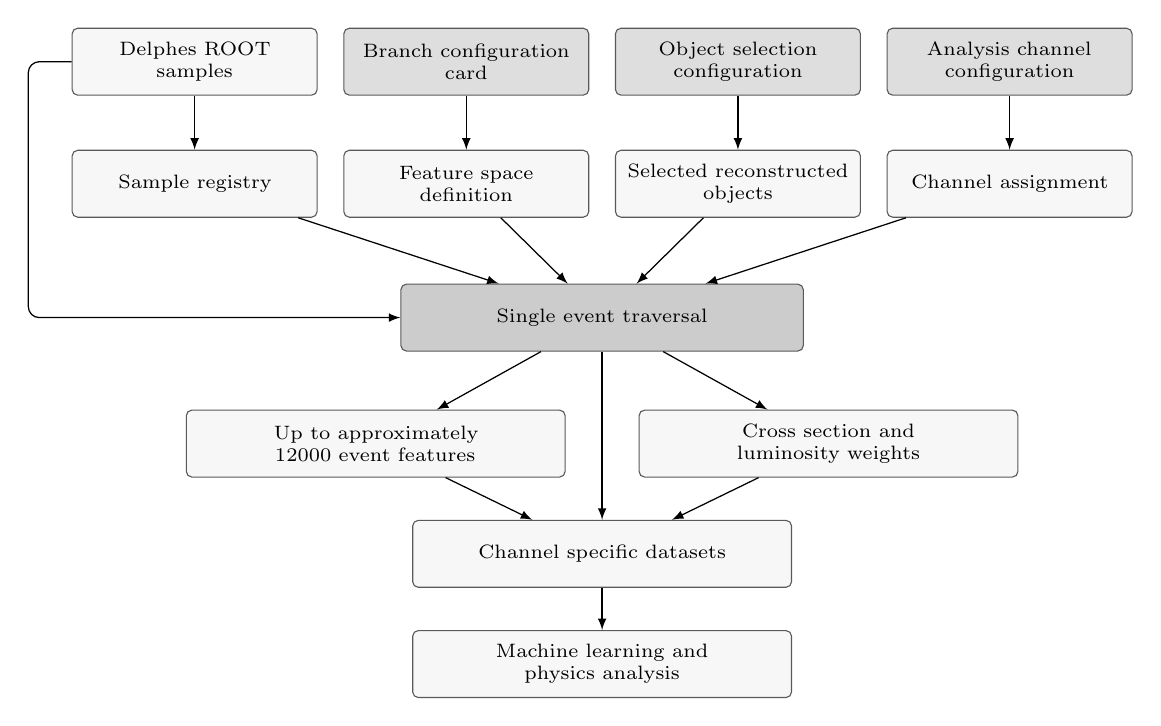
\begin{tikzpicture}[x=1cm,y=1cm]
  % --- sources
  \node[flowbox]  (A) at (0,0)      {Delphes ROOT samples};
  \node[cardbox]  (C) at (3.45,0)   {Branch configuration\\card};
  \node[cardbox]  (E) at (6.90,0)   {Object selection\\configuration};
  \node[cardbox]  (G) at (10.35,0)  {Analysis channel\\configuration};
  % --- derived definitions
  \node[flowbox]  (B) at (0,-1.55)     {Sample registry};
  \node[flowbox]  (D) at (3.45,-1.55)  {Feature space\\definition};
  \node[flowbox]  (F) at (6.90,-1.55)  {Selected reconstructed\\objects};
  \node[flowbox]  (H) at (10.35,-1.55) {Channel assignment};
  % --- hub
  \node[hubbox]   (I) at (5.175,-3.25) {Single event traversal};
  % --- outputs
  \node[broadbox] (J) at (2.30,-4.85)  {Up to approximately\\12000 event features};
  \node[broadbox] (K) at (8.05,-4.85)  {Cross section and\\luminosity weights};
  \node[broadbox] (L) at (5.175,-6.25) {Channel specific datasets};
  \node[broadbox] (M) at (5.175,-7.65) {Machine learning and\\physics analysis};

  % --- vertical pairs
  \foreach \s/\t in {A/B,C/D,E/F,G/H}
    \draw[fl] (\s) -- (\t);

  % --- into the traversal
  \draw[fl] (B) -- (I);
  \draw[fl] (D) -- (I);
  \draw[fl] (F) -- (I);
  \draw[fl] (H) -- (I);

  % samples are also read directly by the traversal; routed clear of the registry
  \coordinate (R) at ($(A.west)+(-0.55,0)$);
  \draw[fl, rounded corners=4pt]
    (A.west) -- (R) -- (R |- I.west) -- (I.west);

  % --- out of the traversal
  \draw[fl] (I) -- (J);
  \draw[fl] (I) -- (K);
  \draw[fl] (I) -- (L);
  \draw[fl] (J) -- (L);
  \draw[fl] (K) -- (L);
  \draw[fl] (L) -- (M);
\end{tikzpicture}
\caption{The current HEPDataset workflow. Configuration cards and the sample
registry define the feature space, the selected reconstructed objects, and the
channel assignment. All of them are consumed in a single traversal of the input
events, which produces the weighted, channel organized datasets that are used
downstream.}
\label{fig:workflow}
\end{figure}

% ---------------------------------------------------------------------
\section{State of the field}

HEPDataset addresses the event representation stage of the analysis lifecycle.
Its input is a ROOT file containing simulated or reconstructed events. The
package can use PyROOT, Uproot, and, in future releases, C++ based event loops to
traverse the input events and extract the requested information. Its target use
case is the construction of event level datasets for an analysis that may use a
multivariate classifier and whose feature space may evolve during the research
process. The central output is not only a yield in a predefined signal region.
It is a reproducible and weighted representation of many individual events with
a large collection of physics motivated features. The event loop can be divided
into independent ranges and executed in parallel before the resulting channel
organized ROOT files are merged. This output can be used to train a BDT, a
neural network, or a future architecture that learns from high dimensional event
information.

The distinction is important for BSM searches. Recasting generally starts with
an analysis whose object definitions and selection regions are already
specified. Machine learning based analysis development can start earlier. The
researcher may wish to retain a wide set of observables and determine through
statistical learning which combinations contain useful information about a
signal hypothesis. The researcher may also wish to compare several signal
regions, mass points, background mixtures, and feature definitions without
rebuilding the entire data production chain.

HEPDataset is therefore complementary to existing HEP software. It does not
attempt to reproduce the detector simulation provided by Delphes. It
does not attempt to replace the analysis validation and recasting capabilities of
MadAnalysis~5, CheckMATE, or Rivet. It provides a configurable data preparation
layer that can supply downstream machine learning frameworks and can later be
connected to statistical tools such as pyhf \citep{pyhf}.

The package is also complementary to generic machine learning libraries.
XGBoost provides scalable gradient boosted decision trees \citep{xgboost}.
HEPDataset does not provide a replacement for XGBoost. It provides a physics
aware method for constructing the input representation that a classifier
requires. Future integrations with attention based and transformer based
architectures can extend this role to models that operate on high dimensional or
structured event representations.

Table~\ref{tab:layers} summarizes the intended division of responsibility.

\begin{table}[htbp]
\centering
\small
\begin{tabular}{@{}>{\raggedright\arraybackslash}p{3.8cm}
                >{\raggedright\arraybackslash}p{6.7cm}
                >{\raggedright\arraybackslash}p{4.2cm}@{}}
\toprule
\textbf{Software layer} & \textbf{Primary responsibility} & \textbf{Role of HEPDataset}\\
\midrule
Event generation       & Production of hard scattering events and decays            & External input\\
Detector simulation    & Approximate detector response and reconstruction           & External input from Delphes\\
Event dataset construction & Selection, feature extraction, weighting, and organization & Primary role\\
Machine learning       & Classification, representation learning, and ranking       & Downstream or planned integration\\
Statistical inference  & Significance estimation and hypothesis testing             & Downstream or planned integration\\
\bottomrule
\end{tabular}
\caption{Intended division of responsibility between HEPDataset and the
surrounding software layers.}
\label{tab:layers}
\end{table}

% ---------------------------------------------------------------------
\section{Software design}

HEPDataset is designed around a separation between the physics description of
the event representation and the operational process that constructs the
dataset. The user specifies the desired objects, observables, channels, regions,
and samples. The package then applies those definitions consistently while
handling event traversal, weighting, parallel execution, temporary output, and
merging. The loop interface is deliberately centered on the input ROOT file and
the channel organized result. A loop can return in memory trees, a dictionary
whose keys identify analysis channels, or paths to ROOT files that have already
been written. This permits PyROOT based, future Uproot based, and future C++
based loop implementations to participate in the same higher level dataset
workflow.

The branch configuration card is the main interface for defining the candidate
feature space. It allows the user to express the physical content of the dataset
without repeatedly modifying the event reading workflow. The card can request
object level quantities and multi object quantities. It can also define the
combinations of objects used for derived variables. This is important because
many discriminative properties of collider events are relational. The invariant
mass of two objects, their angular separation, and their transverse momentum
balance can contain information that is not represented by the individual object
values alone.

The package reads the selected event information and assigns an analysis channel
during the same traversal. The channel representation can distinguish lepton
multiplicity, lepton flavour, charge structure, and jet content. The
configuration in \texttt{analysis\_channels.py} allows the channel taxonomy to
follow the needs of a particular physics analysis. The selection policy in
\texttt{object\_selection.py} provides the corresponding object quality
requirements. Future releases will extend this configurability through dedicated
YAML cards so that object definitions and selection criteria can be recorded as
analysis data rather than only as program logic.

The single traversal design is motivated by both computational and scientific
considerations. Repeated traversal of a large ROOT file increases input output
cost and creates additional opportunities for inconsistent selection. A single
traversal ensures that the features, event category, and event weight are derived
from the same reconstructed event state. It also permits all requested channels
to be produced from the same input pass. The approach is particularly valuable
when the feature space contains thousands of candidate variables.

The processing strategy uses event range partitioning. A ROOT input file is
divided into independent intervals of entries. Each worker receives one interval
and produces isolated temporary outputs. The workers do not write to a common
ROOT file. The resulting files are merged after the workers complete. The
isolation of writes avoids concurrent access conflicts and makes the worker
computation close to embarrassingly parallel. It also provides a clear failure
boundary because a failed interval can be identified without corrupting a shared
output file.

The merging strategy follows the structure of the physics output. Temporary
files are first merged within a sample and channel or region. Sample level
outputs can then be merged into final datasets for the corresponding channel or
region. This hierarchy preserves the provenance of intermediate products while
allowing the user to retain per sample outputs or create combined training
datasets. Temporary files are removed after a successful merge so that the
storage requirement does not grow with the number of processing intervals.

The complete current processing sequence is shown in Figure~\ref{fig:sequence}.

\begin{figure}[t]
\centering
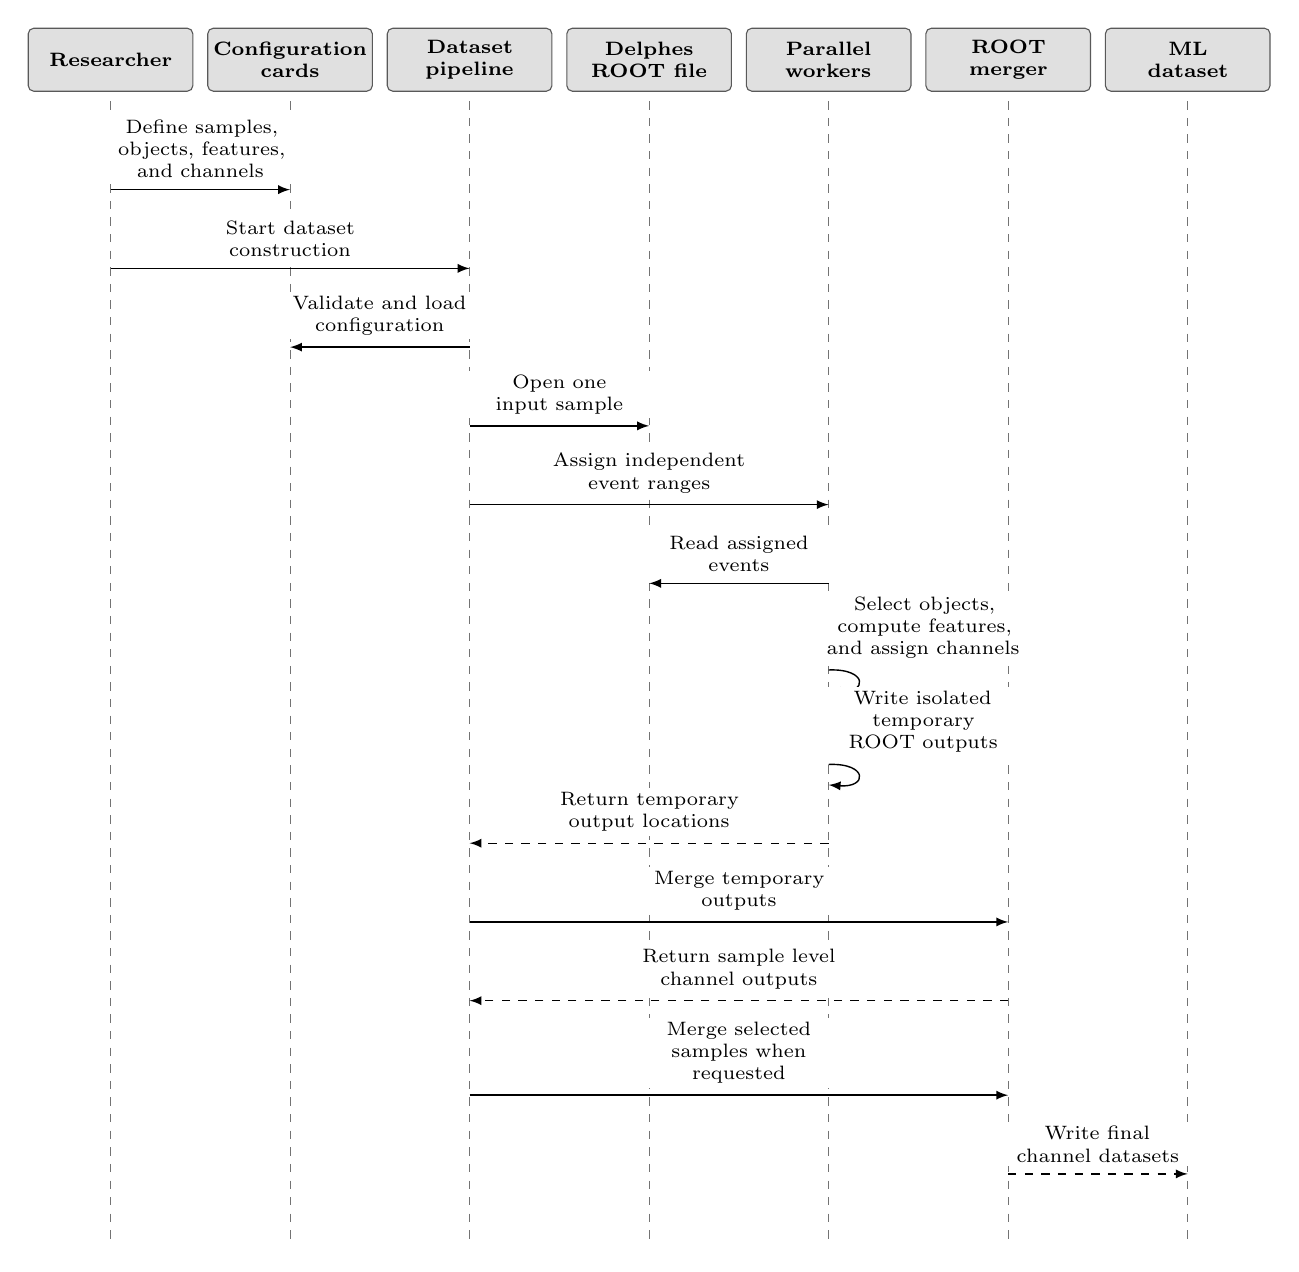
\begin{tikzpicture}[x=1cm,y=1cm]
  % --- participants
  \node[hdrbox] (PU) at (0.00,0)  {Researcher};
  \node[hdrbox] (PC) at (2.28,0)  {Configuration\\cards};
  \node[hdrbox] (PP) at (4.56,0)  {Dataset\\pipeline};
  \node[hdrbox] (PR) at (6.84,0)  {Delphes\\ROOT file};
  \node[hdrbox] (PW) at (9.12,0)  {Parallel\\workers};
  \node[hdrbox] (PH) at (11.40,0) {ROOT\\merger};
  \node[hdrbox] (PO) at (13.68,0) {ML\\dataset};

  % --- lifelines
  \foreach \p in {PU,PC,PP,PR,PW,PH,PO}
    \draw[lifeline] (\p.south) ++(0,-0.12) -- ++(0,-14.5);

  % --- messages
  \msg{0.00}{2.28}{-1.65}{Define samples, objects, features, and channels}{-latex}
  \msg{0.00}{4.56}{-2.65}{Start dataset construction}{-latex}
  \msg{4.56}{2.28}{-3.65}{Validate and load configuration}{-latex}
  \msg{4.56}{6.84}{-4.65}{Open one input sample}{-latex}
  \msg{4.56}{9.12}{-5.65}{Assign independent event ranges}{-latex}
  \msg{9.12}{6.84}{-6.65}{Read assigned events}{-latex}
  \selfmsg{9.12}{-7.75}{Select objects, compute features, and assign channels}
  \selfmsg{9.12}{-8.95}{Write isolated temporary ROOT outputs}
  \msg{9.12}{4.56}{-9.95}{Return temporary output locations}{dashed,-latex}
  \msg{4.56}{11.40}{-10.95}{Merge temporary outputs}{-latex}
  \msg{11.40}{4.56}{-11.95}{Return sample level channel outputs}{dashed,-latex}
  \msg{4.56}{11.40}{-13.15}{Merge selected samples when requested}{-latex}
  \msg{11.40}{13.68}{-14.15}{Write final channel datasets}{dashed,-latex}
\end{tikzpicture}
\caption{The complete current processing sequence, from the configuration and
sample registry through to the merged, channel organized ROOT datasets. Solid
arrows indicate a request and dashed arrows indicate a return.}
\label{fig:sequence}
\end{figure}

The design favors a transparent and configurable data production process over a
fully automatic interpretation of physics intent. The package can calculate
requested observables and apply requested selections. It cannot determine
whether a particular selection is theoretically optimal or whether a variable is
physically appropriate for a given search. That responsibility remains with the
analysis team and requires validation against the detector card, the signal
model, and independent physics calculations.

The package is intended to support two complementary modes of use. In the first
mode, a researcher generates a broad dataset and supplies it to an external
machine learning framework. In the second mode, a future integrated workflow
selects a smaller set of informative features and trains a classifier within the
same analysis environment. The second mode is planned rather than a claim about
the complete current release.

Future development will introduce a discriminative feature selection stage. The
user will be able to define a maximum number of retained features. The selection
stage will seek features that provide strong discrimination between signal and
background while controlling redundancy through an uncorrelatedness requirement.
The purpose is to reduce the high dimensional candidate space to a compact
representation that remains physically interpretable and computationally
manageable.

The planned machine learning and significance workflow is shown in
Figure~\ref{fig:planned}.

\begin{figure}[t]
\centering
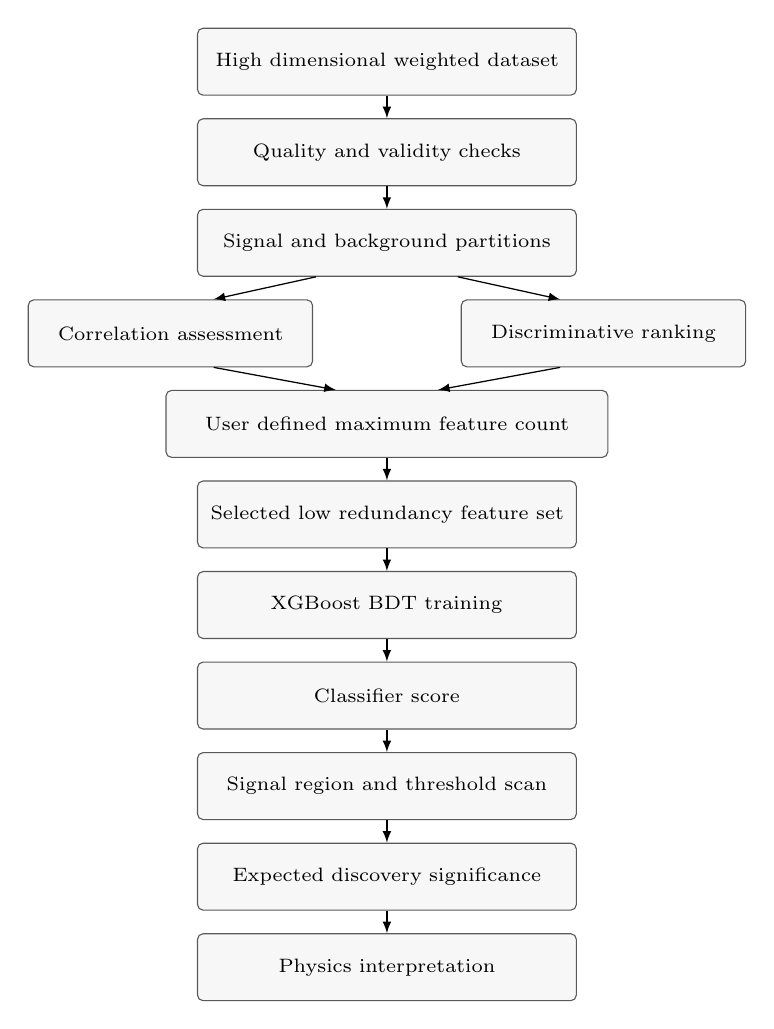
\begin{tikzpicture}[x=1cm,y=1cm]
  \node[broadbox] (A) at (0,0)     {High dimensional weighted dataset};
  \node[broadbox] (B) at (0,-1.15) {Quality and validity checks};
  \node[broadbox] (C) at (0,-2.30) {Signal and background partitions};
  \node[broadbox, text width=3.4cm] (D) at (-2.75,-3.45) {Correlation assessment};
  \node[broadbox, text width=3.4cm] (E) at (2.75,-3.45)  {Discriminative ranking};
  \node[broadbox, text width=5.4cm] (F) at (0,-4.60) {User defined maximum feature count};
  \node[broadbox] (G) at (0,-5.75) {Selected low redundancy feature set};
  \node[broadbox] (H) at (0,-6.90) {XGBoost BDT training};
  \node[broadbox] (I) at (0,-8.05) {Classifier score};
  \node[broadbox] (J) at (0,-9.20) {Signal region and threshold scan};
  \node[broadbox] (K) at (0,-10.35){Expected discovery significance};
  \node[broadbox] (L) at (0,-11.50){Physics interpretation};

  \foreach \s/\t in {A/B,B/C,F/G,G/H,H/I,I/J,J/K,K/L}
    \draw[fl] (\s) -- (\t);
  \draw[fl] ([xshift=-0.9cm]C.south) -- ([xshift=0.55cm]D.north);
  \draw[fl] ([xshift=0.9cm]C.south)  -- ([xshift=-0.55cm]E.north);
  \draw[fl] ([xshift=0.55cm]D.south) -- ([xshift=-0.65cm]F.north);
  \draw[fl] ([xshift=-0.55cm]E.south) -- ([xshift=0.65cm]F.north);
\end{tikzpicture}
\caption{The planned feature selection and significance workflow. Candidate
features are ranked for discrimination and for redundancy against a user defined
maximum feature count before a BDT is trained and the expected discovery
significance is estimated. This stage is planned and complements, rather than
replaces, the high dimensional dataset generator.}
\label{fig:planned}
\end{figure}

This future stage will complement rather than replace the high dimensional
dataset generator. The broad dataset remains the important scientific product
because it permits the use of advanced learning systems that can discover
nonlinear and higher order relationships among many observables. Feature
reduction provides an optional route for interpretable BDT based studies and for
applications where computational cost or systematic control favors a smaller
representation.

% ---------------------------------------------------------------------
\section{Research impact statement}

HEPDataset is intended to reduce the time required to move from Delphes
detector simulation to an analysis ready machine learning dataset. Its impact is
therefore measured not only by the number of features or processed events. It is
measured by whether analysis groups can construct, modify, validate, and compare
event representations with less duplicated engineering effort.

The package can support searches for BSM physics in which the signal is
distributed across several correlated kinematic properties. A conventional cut
based analysis may use a small number of observables selected from prior physical
intuition. HEPDataset permits the analyst to retain a substantially broader
candidate space before the final classifier architecture or feature selection
procedure is chosen. This is relevant for signals with complex decay chains,
multiple production modes, compressed spectra, or experimentally overlapping
final states.

The package also supports reproducible comparison between analyses. The branch
configuration card records the requested feature space. The sample registry
records the input processes and cross sections. The channel and object selection
descriptions record the event categorization. Together these inputs provide a
more explicit account of the data construction process than a collection of
disconnected analysis scripts.

The planned feature selection and XGBoost integration will enable a complete
exploratory workflow in which candidate variables are ranked, a BDT is trained,
and the classifier score is used to estimate expected discovery significance for
BSM signals. Such a workflow can help identify promising signal models and guide
the design of later analysis selections. The significance estimate will remain
dependent on the statistical model, systematic uncertainties, signal and
background normalization, and assumptions about the dataset. It will therefore
be an analysis aid rather than an automatic claim of discovery sensitivity.

The broader objective is to make the rapid generation of high dimensional event
datasets routine. The resulting datasets can be supplied to advanced machine
learning systems that exploit thousands of input features. Architectures based
on attention and transformer mechanisms may learn relationships among event
observables that are difficult to encode through manual feature selection.
HEPDataset provides the data preparation foundation for these studies while
preserving the possibility of using established classifiers such as XGBoost.

The software is intended for research use in collider phenomenology and machine
learning based HEP analysis. Its outputs should be validated using independent
physics calculations, controlled samples, closure tests, and systematic
uncertainty studies before they are used for a physics claim. The project will
benefit from future contributions that improve configuration validation, add
dedicated selection cards, test serial and parallel equivalence, expand output
format support, and connect the feature generation stage to modern high
dimensional learning architectures.

% ---------------------------------------------------------------------
\section{AI usage disclosure}

Generative artificial intelligence was used to assist with the revision of this
manuscript. The assistance was limited to restructuring prose, improving academic
language, and organizing the description of the software according to the
requested Journal of Open Source Software sections. The repository source files,
configuration examples, existing manuscript, and stated software behavior were
reviewed by the authors before the revised text was prepared. Claims concerning
current functionality were constrained to behavior represented in the repository.
Planned feature selection, classifier training, and discovery significance
functionality are explicitly described as future developments rather than as
capabilities of the current release. The authors remain responsible for the
scientific accuracy, completeness, and final content of this manuscript.

% ---------------------------------------------------------------------
% References
%
% The four entries are reproduced here so that this file stands alone and so
% that acronyms in the titles (ROOT, XGBoost, HistFactory) keep their case,
% which the installed BibTeX styles do not preserve.  The citation keys and
% author-year labels match paper.bib; to generate the list from that file
% instead, replace this block with
%     \bibliographystyle{plainnat}
%     \bibliography{paper}
% and protect the acronyms in paper.bib with braces.
% ---------------------------------------------------------------------
\begin{thebibliography}{1}

\bibitem[Brun and Rademakers(1997)]{root}
R.~Brun and F.~Rademakers.
\newblock {ROOT} -- an object oriented data analysis framework.
\newblock \emph{Nuclear Instruments and Methods in Physics Research Section A},
  389(1--2):81--86, 1997.
\newblock doi: \href{https://doi.org/10.1016/S0168-9002(97)00048-X}{10.1016/S0168-9002(97)00048-X}.

\bibitem[Chen and Guestrin(2016)]{xgboost}
Tianqi Chen and Carlos Guestrin.
\newblock {XGBoost}: a scalable tree boosting system.
\newblock In \emph{Proceedings of the 22nd ACM SIGKDD International Conference
  on Knowledge Discovery and Data Mining}, pages 785--794, 2016.
\newblock doi: \href{https://doi.org/10.1145/2939672.2939785}{10.1145/2939672.2939785}.

\bibitem[de Favereau et~al.(2014)]{delphes}
J.~de Favereau, C.~Delaere, P.~Demin, A.~Giammanco, V.~Lema\^itre, A.~Mertens,
  and M.~Selvaggi.
\newblock {DELPHES} 3: a modular framework for fast simulation of a generic
  collider experiment.
\newblock \emph{Journal of High Energy Physics}, 2014(2):57, 2014.
\newblock doi: \href{https://doi.org/10.1007/JHEP02(2014)057}{10.1007/JHEP02(2014)057}.

\bibitem[Heinrich et~al.(2021)]{pyhf}
Lukas Heinrich, Matthew Feickert, Giordon Stark, and Kyle Cranmer.
\newblock {pyhf}: pure-{Python} implementation of {HistFactory} statistical
  models.
\newblock \emph{Journal of Open Source Software}, 6(58):2823, 2021.
\newblock doi: \href{https://doi.org/10.21105/joss.02823}{10.21105/joss.02823}.

\end{thebibliography}

\end{document}
